\documentclass[10pt,a4paper]{article}

% ---------- Research-paper formatting ----------
\usepackage[margin=22mm]{geometry}
\usepackage[T1]{fontenc}
\usepackage{lmodern}
\usepackage{microtype}
\usepackage{amsmath,amssymb}
\usepackage{booktabs,tabularx,array}
\usepackage{graphicx}
\usepackage{xcolor}
\definecolor{navy}{HTML}{17324D}
\definecolor{blue}{HTML}{2878B5}
\definecolor{teal}{HTML}{1B998B}
\definecolor{gold}{HTML}{E3A72F}
\definecolor{coral}{HTML}{D9655B}
\definecolor{paleBlue}{HTML}{EAF3FA}
\definecolor{paleTeal}{HTML}{E8F6F3}
\definecolor{paleGold}{HTML}{FFF5DD}
\definecolor{paleCoral}{HTML}{FBECEA}
\usepackage{tikz}
\usetikzlibrary{arrows.meta,positioning,calc,fit,shapes.geometric,shadows}
\usepackage{caption}
\usepackage[hidelinks]{hyperref}
\usepackage{enumitem}
\usepackage[section]{placeins}
\graphicspath{{figures/}}
\newcommand{\ind}{\mathbb{I}}
\setlength{\textfloatsep}{14pt plus 2pt minus 2pt}
\setlength{\floatsep}{12pt plus 2pt minus 2pt}
\setcounter{topnumber}{3}
\renewcommand{\topfraction}{0.9}
\renewcommand{\textfraction}{0.08}
\renewcommand{\floatpagefraction}{0.75}
\setlength{\parindent}{1em}
\setlength{\parskip}{2pt}
\setlength{\emergencystretch}{2em}
\captionsetup{font=small,labelfont=bf}
\setlist{nosep,leftmargin=*}
\newcommand{\R}{\mathbb{R}}
\newcommand{\model}[1]{\texttt{\small #1}}

\title{\textbf{CulturalQA: Retrieval-Augmented Question Answering for Underrepresented Cultural Knowledge}\\
\large A Controlled Study of Mixture-of-Experts Reranking}
\author{
\small
\begin{tabular}[t]{c}
\textbf{Kashvi Ranjan} (230911056) \quad
\textbf{Venisa Tellis} (230911064) \quad
\textbf{P. Manisha} (230911106)
\end{tabular}
}
\date{}

\begin{document}
\maketitle

\begin{abstract}
Underrepresented cultural knowledge can be difficult to answer reliably using language models alone. We present CulturalQA, a grounded question-answering system built over 74,528 records from five cultural resources: DOSA, SCALE, DRISHTIKON, DIWALI, and the Indian Cultural Dataset. The pipeline combines multilingual dense retrieval, BM25, weighted reciprocal-rank fusion, query expansion, cross-encoder reranking, and an extractive reader; a separate CLIP pathway retrieves existing images. We evaluate whether a learned text--image Mixture-of-Experts (MoE) fusion score improves the cross-encoder ranking. The MoE uses frozen BERT and CLIP features, one shared expert, and three routed experts. In a matched saved-candidate replay of 100 factual questions, adding the MoE score reduced top-3 Exact Match from 65\% to 63\% and F1 from 68.57\% to 66.57\%; at top 6, both conditions achieved 60\% Exact Match. These results do not show a benefit from the current MoE design. We recommend the cross-encoder baseline for this benchmark and discuss limitations including weak supervision, a previously inspected evaluation set, one training seed, and incomplete indexing of long records.
\end{abstract}

\noindent\textbf{Keywords:} cultural question answering; retrieval-augmented generation; hybrid retrieval; cross-encoder; mixture of experts; multimodal fusion.

\section{Introduction}
Questions about regional festivals, artifacts, rituals, clothing, food, and vocabulary require reliable, traceable cultural information. Language models can produce fluent but unsupported answers, particularly where source coverage is limited. Retrieval-augmented question answering addresses this problem by grounding responses in searchable evidence \cite{rag}.

CulturalQA searches five cultural datasets, reranks candidate records, and extracts an answer span from retrieved text. Image requests use a separate CLIP-based retrieval path \cite{clip}. Our research focus is whether a learned multimodal Mixture-of-Experts (MoE) relevance signal improves a strong cross-encoder baseline. The study asks:
\begin{enumerate}
\item Does MoE reranking improve evidence ranking and answer quality?
\item On which sources or questions do rankings change, and are changes beneficial?
\item What additional processing cost does MoE introduce?
\end{enumerate}

\textbf{Contributions.} We document a five-source grounded-QA pipeline; describe a shared/routed multimodal MoE reranker; compare the baseline and MoE-augmented ranking on a common saved candidate pool; and report the negative result alongside the evaluation limitations.

\textbf{Scope.} This is a saved-candidate replay, not a fresh end-to-end or blind evaluation. Candidate retrieval, cached query formulations, and per-context reader outputs are shared between conditions; the ranking scores and resulting evidence selection are recomputed.

\section{Related Work}
Retrieval-augmented generation grounds model responses in retrieved passages \cite{rag}. Dense sentence encoders support semantic matching \cite{sbert}, while BM25 helps match exact names and terminology \cite{bm25}. Reciprocal-rank fusion combines ranked lists without requiring directly comparable scores \cite{rrf}; FAISS supports efficient vector search \cite{faiss}.

Cross-encoders jointly score query--passage pairs and are widely used for reranking \cite{monobert,msmarco}. Extractive readers predict answer spans and can be trained to abstain when evidence is insufficient \cite{roberta,squad1,squad2}. MoE architectures use a gate to assign input-dependent weights to expert networks \cite{shazeer,switch}. Multimodal fusion can use concatenation, attention, tensor interactions, or element-wise products \cite{tfn,lmf}. CLIP provides image representations and text-to-image similarity \cite{clip}. CulturalQA combines these ideas in a smaller relevance-ranking model rather than a generative multimodal QA model.

\section{Dataset and Preprocessing}
The active corpus contains five resources. Counts below are from the local research manifest and should not be interpreted as publisher-reported dataset totals.

\begin{table}[htbp]
\centering
\small
\caption{Local corpus inventory.}
\label{tab:data}
\begin{tabularx}{\linewidth}{@{}l r X@{}}
\toprule
\textbf{Dataset} & \textbf{Records} & \textbf{Content and modality}\\
\midrule
DOSA & 630 & Artifact clues and state metadata; text\\
SCALE & 695 & Cultural items, translations, and domains; text\\
DRISHTIKON & 64,290 & Questions, answers, attributes, and image references; text and images\\
DIWALI & 8,817 & Region-specific concepts and descriptions; text\\
Indian Cultural Dataset & 96 & Descriptive cultural text and category\\
\midrule
\textbf{Total} & \textbf{74,528} & \textbf{Five active sources}\\
\bottomrule
\end{tabularx}
\end{table}

DOSA and SCALE are obtained from their respective Microsoft and Google Research repositories; DIWALI, DRISHTIKON, and the Indian Cultural Dataset are hosted on Hugging Face \cite{dosa,scale,diwali,drishtikon,icd}. SCALE includes international cultural material, so the corpus is not exclusively Indian. DRISHTIKON is the only active source with record-associated images; the local audit found 1,549 image paths and 1,536 distinct image-byte contents.

CSV, JSON/JSONL, Excel, and report files are loaded with source IDs and metadata preserved. Records are serialized into labelled text; DRISHTIKON distractor options are retained as structured fields but omitted from searchable text. Image names are resolved against local files, and byte-identical images are grouped. Long reports are chunked into 900-character passages with 150-character overlap; records over 4,000 characters use 1,200-character chunks with 200-character overlap. A 15-chunk cap is applied to long records.

The active index contains 75,752 searchable documents, including 122 report chunks. Coverage is not complete for every record: the Indian Cultural Dataset has only 4.24\% of source characters indexed, with 11 of 96 records fully indexed. This limitation is relevant when interpreting retrieval and answer scores.

\section{Methodology}
\subsection{System Overview}
CulturalQA supports exact-record lookup, factual text answering, list retrieval, and standalone image retrieval. For factual questions, retrieval and ranking select evidence; the extractive reader returns a span from selected text or abstains. It does not generate free-form answers.

\begin{figure}[htbp]
\centering
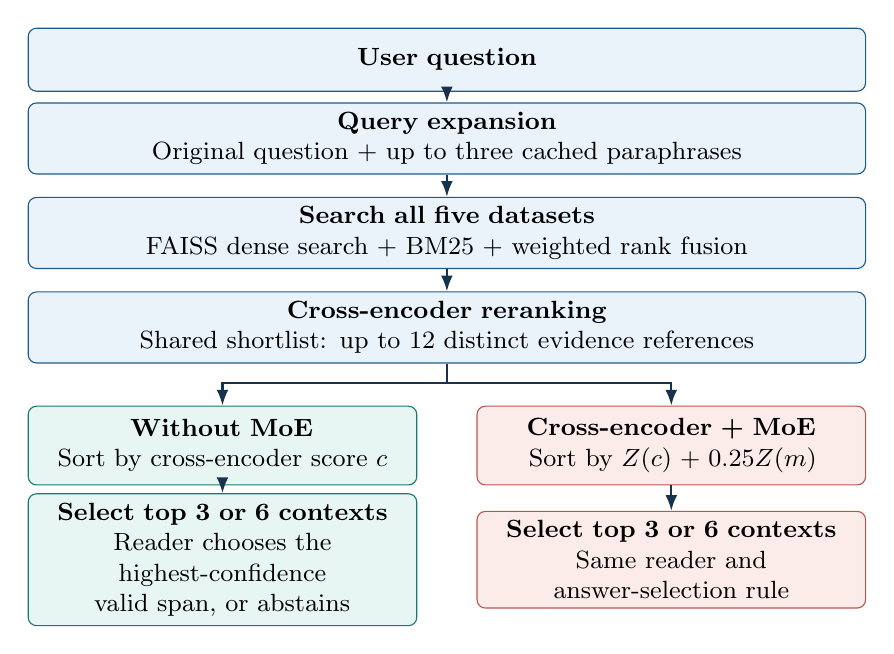
\begin{tikzpicture}[
 stage/.style={draw=blue!75!black,fill=paleBlue,rounded corners=3pt,
 align=center,text width=10.4cm,minimum height=8mm,font=\small},
 base/.style={draw=teal!80!black,fill=paleTeal,rounded corners=3pt,
 align=center,text width=4.7cm,minimum height=10mm,font=\small},
 moe/.style={draw=coral!85!black,fill=paleCoral,rounded corners=3pt,
 align=center,text width=4.7cm,minimum height=10mm,font=\small},
 arr/.style={-{Latex[length=2mm]},thick,draw=navy}]
\node[stage] (q) at (0,0) {\textbf{User question}};
\node[stage] (exp) at (0,-1.0) {\textbf{Query expansion}\\Original question + up to three cached paraphrases};
\node[stage] (retr) at (0,-2.2) {\textbf{Search all five datasets}\\FAISS dense search + BM25 + weighted rank fusion};
\node[stage] (ce) at (0,-3.4) {\textbf{Cross-encoder reranking}\\Shared shortlist: up to 12 distinct evidence references};
\node[base] (base) at (-2.85,-4.9) {\textbf{Without MoE}\\Sort by cross-encoder score $c$};
\node[moe] (moe) at (2.85,-4.9) {\textbf{Cross-encoder + MoE}\\Sort by $Z(c)+0.25Z(m)$};
\node[base] (rbase) at (-2.85,-6.35) {\textbf{Select top 3 or 6 contexts}\\Reader chooses the highest-confidence valid span, or abstains};
\node[moe] (rmoe) at (2.85,-6.35) {\textbf{Select top 3 or 6 contexts}\\Same reader and answer-selection rule};
\draw[arr] (q)--(exp); \draw[arr] (exp)--(retr); \draw[arr] (retr)--(ce);
\draw[arr] (ce.south)--++(0,-0.25)-|(base.north);
\draw[arr] (ce.south)--++(0,-0.25)-|(moe.north);
\draw[arr] (base)--(rbase); \draw[arr] (moe)--(rmoe);
\end{tikzpicture}
\caption{Factual-answering workflow. The saved-candidate comparison shares retrieval candidates, cached query formulations, and per-context reader outputs; only the ranking policy and resulting evidence selection differ. The diagram describes the operational flow; the replay reuses the recorded retrieval and reader outputs.}
\label{fig:architecture}
\end{figure}

\subsection{Hybrid Retrieval}
The retrieval encoder is \model{sentence-transformers/paraphrase-multilingual-MiniLM-L12-v2}, producing 384-dimensional vectors:
\begin{equation}
\mathbf{u}_{q}=E_{\mathrm{ret}}(q),\qquad
\mathbf{u}_{d}=E_{\mathrm{ret}}(d),\qquad \mathbf{u}_{q},\mathbf{u}_{d}\in\R^{384}.
\end{equation}
FAISS uses squared Euclidean distance on stored vectors without explicit normalization. BM25 complements dense retrieval by matching explicit terms:
\begin{equation}
\mathrm{BM25}(q,d)=\sum_{w\in q}\mathrm{IDF}(w)
\frac{f(w,d)(k_1+1)}
{f(w,d)+k_1(1-b+b|d|/\overline{|d|})}.
\end{equation}
Dense and lexical rankings are merged using weighted reciprocal-rank fusion:
\begin{equation}
\mathrm{RRF}(d)=
\sum_{r\in\{\mathrm{dense},\mathrm{BM25}\}}
\frac{w_r}{60+\mathrm{rank}_r(d)},\quad
w_{\mathrm{dense}}=0.6,\quad w_{\mathrm{BM25}}=0.4.
\end{equation}
Each dataset branch requests eight dense and eight sparse results per formulation. A dataset hint adjusts a branch's budget and weight but does not exclude the other sources.

For query expansion, \model{openai/gpt-oss-20b} is accessed through Groq at temperature zero to propose up to three paraphrases. The original question is retained, duplicates are removed, and results are cached. The cross-encoder \model{cross-encoder/ms-marco-MiniLM-L-6-v2} scores the original question against the pooled candidates. Deduplication by dataset and evidence reference produces a common shortlist of up to 12 candidates. Both experimental conditions rerank this same shortlist and return the top $K\in\{3,6\}$ contexts.

\subsection{Multimodal Representations and MoE}
The fusion model uses frozen \model{bert-base-uncased} \cite{bert} and \model{openai/clip-vit-base-patch32} encoders. BERT supplies its pooled classification-token representation, using a 256-token limit, as a 768-dimensional text vector, while CLIP produces a 512-dimensional image vector; if an image is unavailable, a zero vector is used. Learned affine projections map both to 256 dimensions:
\begin{equation}
\mathbf{t}=W_t\mathbf{h}_t+\mathbf{b}_t,\qquad
\mathbf{v}=W_v\mathbf{h}_v+\mathbf{b}_v,\qquad
\mathbf{t},\mathbf{v}\in\R^{256}.
\end{equation}
Before fusion, text and image have separate vectors. Fusion is tested because text captures names and cultural descriptions, while images may contribute appearance and visual context. The QA reader remains text-only; image information can affect which textual evidence is ranked and passed to it.

The model has one always-active shared concatenation expert and three routed experts. The shared expert transforms the concatenated vectors. The routed experts model (i) attention between pooled text and image vectors, (ii) low-rank bilinear/tensor interactions, and (iii) element-wise multiplication. Each expert returns a 256-dimensional vector. These are alternative interaction functions, not separately pretrained QA models.

\begin{figure}[htbp]
\centering
\resizebox{0.97\linewidth}{!}{%
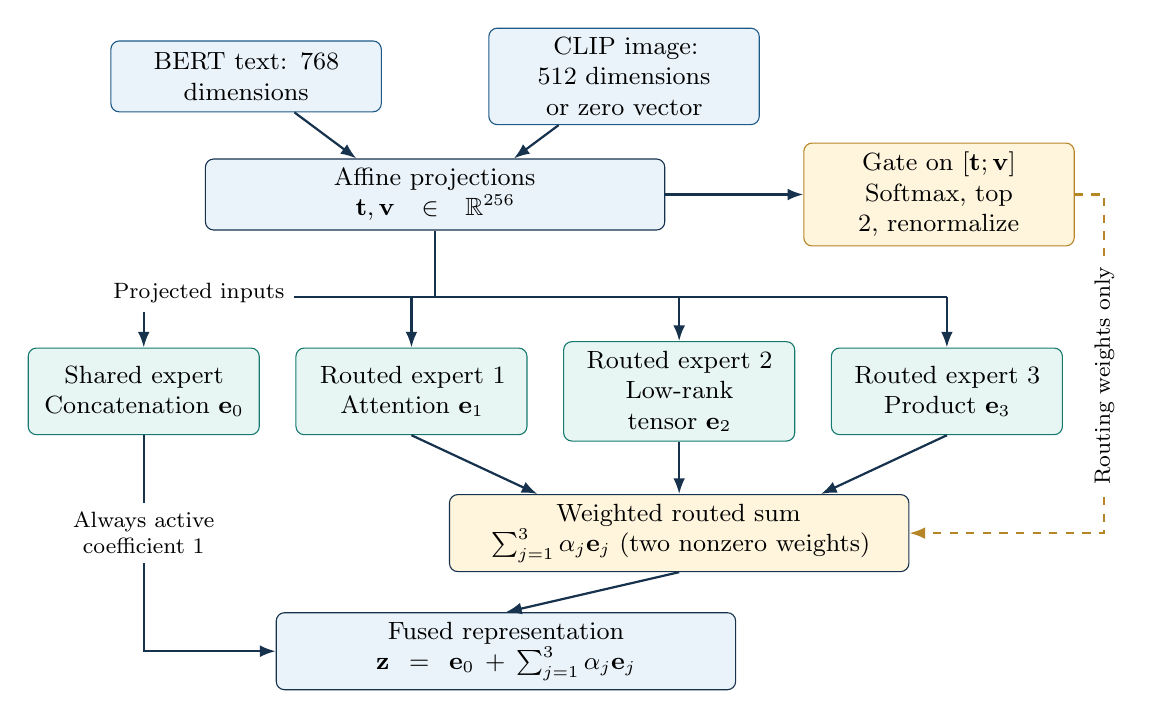
\begin{tikzpicture}[
 b/.style={draw=blue!75!black,fill=paleBlue,rounded corners=3pt,
 align=center,text width=3.2cm,minimum height=9mm,font=\small},
 e/.style={draw=teal!80!black,fill=paleTeal,rounded corners=3pt,
 align=center,text width=2.7cm,minimum height=11mm,font=\small},
 w/.style={draw=navy,fill=white,rounded corners=3pt,
 align=center,text width=5.6cm,minimum height=9mm,font=\small},
 arr/.style={-{Latex[length=2mm]},thick,draw=navy}]
\node[b] (text) at (-3.8,1.0) {BERT text: 768 dimensions};
\node[b] (image) at (1.0,1.0) {CLIP image: 512 dimensions\\or zero vector};
\node[w,fill=paleBlue] (p) at (-1.4,-0.5) {Affine projections\\$\mathbf t,\mathbf v\in\R^{256}$};
\node[b,fill=paleGold,draw=gold!80!black] (g) at (5.0,-0.5) {Gate on $[\mathbf t;\mathbf v]$\\Softmax, top 2, renormalize};
\node[e] (e0) at (-5.1,-3.0) {Shared expert\\Concatenation $\mathbf e_0$};
\node[e] (e1) at (-1.7,-3.0) {Routed expert 1\\Attention $\mathbf e_1$};
\node[e] (e2) at (1.7,-3.0) {Routed expert 2\\Low-rank tensor $\mathbf e_2$};
\node[e] (e3) at (5.1,-3.0) {Routed expert 3\\Product $\mathbf e_3$};
\node[w,fill=paleGold] (mix) at (1.7,-4.8) {Weighted routed sum\\$\sum_{j=1}^{3}\alpha_j\mathbf e_j$ (two nonzero weights)};
\node[w,fill=paleBlue] (out) at (-0.5,-6.3) {Fused representation\\$\mathbf z=\mathbf e_0+\sum_{j=1}^{3}\alpha_j\mathbf e_j$};
\draw[arr] (text)--([xshift=-1cm]p.north);
\draw[arr] (image)--([xshift=1cm]p.north);
\draw[arr] (p.east)--(g.west);
\draw[thick,navy] (p.south)--(-1.4,-1.8);
\draw[thick,navy] (-5.1,-1.8)--(5.1,-1.8);
\foreach \x/\n in {-5.1/e0,-1.7/e1,1.7/e2,5.1/e3}{\draw[arr] (\x,-1.8)--(\n.north);}
\node[font=\footnotesize,fill=white] at (-4.4,-1.75) {Projected inputs};
\draw[arr] (e1.south)--([xshift=-1.8cm]mix.north);
\draw[arr] (e2.south)--(mix.north);
\draw[arr] (e3.south)--([xshift=1.8cm]mix.north);
\draw[arr,dashed,draw=gold!80!black] (g.east)--(7.1,-0.5)--(7.1,-4.8)--(mix.east);
\node[font=\footnotesize,rotate=90,fill=white] at (7.1,-2.8) {Routing weights only};
\draw[arr] (e0.south)--(-5.1,-6.3)--(out.west);
\node[font=\footnotesize,align=center,fill=white] at (-5.1,-4.8) {Always active\\coefficient 1};
\draw[arr] (mix.south)--(out.north);
\end{tikzpicture}}
\caption{MoE data flow. Solid arrows carry representations; the dashed arrow carries routing weights. Every expert receives projected inputs directly. The shared expert bypasses gating, while the gate weights only the routed sum. All routed outputs are computed before selecting two contributions. Fusion is applied separately to the question and each candidate.}
\label{fig:moe}
\end{figure}

The gate computes probabilities from the concatenated input:
\begin{equation}
\boldsymbol{\ell}=W_g[\mathbf{t};\mathbf{v}]+\mathbf{b}_g,\qquad
p_j=\frac{\exp(\ell_j)}{\sum_{r=1}^{3}\exp(\ell_r)}.
\end{equation}
It retains the two highest probabilities and renormalizes them:
\begin{equation}
\mathcal S=\operatorname{Top2}(\mathbf p),\qquad
\alpha_j=\begin{cases}p_j/\sum_{r\in\mathcal S}p_r,&j\in\mathcal S,\\0,&j\notin\mathcal S.\end{cases}
\end{equation} The fused representation is
\begin{equation}
\mathbf{z}=\mathbf{e}_0+\sum_{j=1}^{3}\alpha_j\mathbf{e}_j,\qquad
\mathbf{z}\in\R^{256}.
\end{equation}
The routed weights sum to one, while the shared expert is added with coefficient one. The weights are learned through the relevance objective; they express each expert's contribution to the representation, not answer confidence. Although only two routed experts contribute, all three routed outputs are computed in the current implementation.

For a text-only record, the image input is zero and its projection becomes a learned constant. The gate can still combine text transformations, but no visual evidence is added. Since only DRISHTIKON supplies record-associated images, multimodal benefit is a hypothesis rather than an assumption.

\subsection{Ranking Conditions and Answer Extraction}
Question and candidate representations are fused separately:
\begin{equation}
\mathbf z_q=F(E_{\mathrm{BERT}}(q),\mathbf0),\qquad
\mathbf z_d=F(E_{\mathrm{BERT}}(d),\mathbf h_{v,d}),\qquad
m(q,d)=\frac{\mathbf z_q^\top\mathbf z_d}{\|\mathbf z_q\|_2\|\mathbf z_d\|_2}.
\end{equation}
The question has no image input. A candidate uses its associated image when available; otherwise its image input is zero. The baseline ranks by the cross-encoder score $c(q,d)$. For each question's common shortlist of $M\leq12$ candidates, scores are standardized separately within that shortlist:
\begin{equation}
Z(x_j)=\frac{x_j-\bar x}{\max(\sigma_x,10^{-6})},\qquad
\sigma_x=\sqrt{\frac{1}{M}\sum_{r=1}^{M}(x_r-\bar x)^2}.
\end{equation}
The unrestricted augmented condition uses
\begin{equation}
s(q,d)=Z(c(q,d))+\lambda Z(m(q,d)),\qquad\lambda=0.25.
\end{equation}
Any candidate in the shortlist can change position and enter or leave the final top $K$. Exact ties retain the cross-encoder order. The development-selected $\lambda$ mixes two relevance scores; it is distinct from the input-dependent expert weights $\alpha_j$. The fusion model has 1,200,451 trainable parameters; pretrained encoders remain frozen.

The reader is \model{deepset/roberta-base-squad2}. It evaluates each selected context separately, using 384-token windows with stride 128. Eligible spans contain only context tokens and at most 30 tokens. Within each window it selects the eligible span maximizing the sum of start and end logits (equivalently, their probability product under fixed normalization):
\begin{equation}
(i^*,j^*)=\arg\max_{\substack{i\leq j,\ j-i+1\leq30\\i,j\text{ eligible context positions}}}
\{\ell_s(i)+\ell_e(j)\}.
\end{equation}
A span is rejected if the null-position logit sum exceeds the span's logit sum. Retained-span confidence is the product of start and end probabilities normalized over eligible context positions plus the null position. The highest-confidence valid span across windows and selected contexts is returned, subject to a minimum score of 0.01; otherwise the system abstains. Confidence is a selection score, not a calibrated correctness probability. Both conditions use these same rules and cached per-context outputs.

\subsection{Separate Image Retrieval}
Standalone image queries use CLIP text-to-image cosine similarity:
\begin{equation}
s_{\mathrm{image}}(q,I)=\cos(E_{\mathrm{CLIP,text}}(q),E_{\mathrm{CLIP,image}}(I)).
\end{equation}
This path returns existing images and metadata; it does not generate a visual answer. The image-pool setting is related to RetVQA \cite{retvqa}, whose method uses a learned relevance encoder and Multi-Image BART for answer generation from retrieved images. CulturalQA uses CLIP retrieval and a text-only extractive reader, so it does not reproduce that paper's full visual-answering architecture. The standalone image path does not use the MoE reranker compared here.

\section{Experimental Setup}
\subsection{Source-group Split and Supervision}
Records are grouped by artifact or concept names, SCALE terms, exact long-document content, and image identity before allocating approximately 70\%, 15\%, and 15\% of groups to training, development, and testing with seed 42. Exact image-byte aliases share a fold, with cross-fold aliases moved to the furthest-held-out fold. This removes exact image-content overlap without claiming to remove every semantic or visual near duplicate. The resulting record populations are shown in Table~\ref{tab:split}.

\begin{table}[htbp]
\centering\small
\caption{Source-group fold populations. These are record counts, not the smaller anchor sets used to train the reranker.}
\label{tab:split}
\begin{tabular}{@{}lrrr@{}}
\toprule Dataset & Train & Development & Test\\\midrule
DOSA & 439 & 95 & 96\\
SCALE & 486 & 104 & 105\\
DRISHTIKON & 45,102 & 9,286 & 9,902\\
DIWALI & 6,175 & 1,306 & 1,336\\
Indian Cultural Dataset & 67 & 14 & 15\\\midrule
Total & 52,269 & 10,805 & 11,454\\\bottomrule
\end{tabular}
\end{table}

All active knowledge documents remain searchable, including evidence for held-out query groups. The separation concerns supervision for the trained reranker, rather than removal of test-time knowledge from the search index. Training uses 300 source-derived anchors (60 per dataset); development uses 60 (12 per dataset), with one anchor per source group. Each anchor is paired with its source record and a sampled negative from a different group and normalized question. Negative sampling alternates between eligible same-dataset and pooled records; pooled negatives can also come from the same dataset. Labels are weak: sampled negatives are not exhaustively judged irrelevant. Query image inputs are zero; positive and negative records use their own images when available.

\subsection{Training Objectives and Model Selection}
Only the projections and fusion network are trained. Initial training uses the triplet objective
\begin{equation}
\mathcal L_{\mathrm{trip}}=\frac1B\sum_{i=1}^B
\max\{0,0.2-\cos(\mathbf z_{q_i},\mathbf z_{p_i})+\cos(\mathbf z_{q_i},\mathbf z_{n_i})\}.
\end{equation}
A balancing term penalizes unequal mean routing probabilities:
\begin{equation}
\mathcal L_{\mathrm{bal}}=\frac13\sum_{j=1}^3(\bar p_j-1/3)^2,
\qquad \bar p_j=\frac1B\sum_i p_{ij}.
\end{equation}
The initial loss is $\mathcal L_{\mathrm{trip}}+0.01\mathcal L_{\mathrm{bal}}$, averaging the balancing term over query, positive, and negative passes. Adam training runs for eight epochs at learning rate $10^{-3}$, batch size 32, and seed 42. The initial checkpoint is selected at epoch 6 by minimum development triplet hinge loss.

Listwise refinement uses the same 300 anchors and 60 development anchors. For query $i$, $\mathcal E_i$ contains its positive and eligible candidate positives from other training anchors whose groups and normalized questions differ:
\begin{equation}
\mathcal L_{\mathrm{list}}=-\frac1N\sum_{i=1}^N\log
\frac{\exp(\cos(\mathbf z_{q_i},\mathbf z_{d_i})/T)}
{\sum_{j\in\mathcal E_i}\exp(\cos(\mathbf z_{q_i},\mathbf z_{d_j})/T)}.
\end{equation}
The refinement objective adds balancing loss averaged over query and candidate passes with coefficient 0.01. Trials consider fresh or triplet-checkpoint initialization and $T\in\{0.05,0.1\}$. Training uses full batches of 300, AdamW at $10^{-4}$, weight decay 0.01, gradient clipping at norm 1, and 20 epochs.

Diagnostic development shortlists contain an injected positive and 11 eligible BERT-selected negatives. Checkpoints are retained by development MRR@12, then Hit@3; residual-score ties prefer a smaller ranking coefficient, and unchanged scores retain the earlier epoch. Final selection uses actual global retrieval for all 60 development queries, without positive injection, and tries $\lambda\in\{0,0.05,0.1,0.25,0.5,1,2\}$. It maximizes MRR@12, then Hit@3, then prefers smaller $\lambda$. The selected model starts from the triplet checkpoint, uses $T=0.1$, retains refinement epoch 20, and uses $\lambda=0.25$. Development data are reused across selection stages, so development scores are not unbiased generalization estimates.

\begin{table}[htbp]
\centering\small
\caption{Additional reproducibility settings. Training and selection settings are specified in the text.}
\label{tab:settings}
\begin{tabularx}{\linewidth}{@{}lX@{}}
\toprule Setting & Value\\\midrule
Text / image / fusion dimensions & 768 / 512 / 256\\
Shared / routed / selected routed experts & 1 / 3 / 2\\
Attention heads / low-rank interaction width & 4 / 32\\
BERT limit / training record-text cap & 256 tokens / 2,000 characters\\
Dense / sparse branch budget & 8 each per formulation; doubled for a hinted dataset\\
RRF weights / constant & 0.6 dense, 0.4 sparse / 60\\
Common shortlist / final evidence & Up to 12 / top 3 or 6\\
Reader length / stride / maximum span & 384 / 128 / 30 tokens\\
Null-difference threshold / minimum score & 0 / 0.01\\
Seed / training CPU threads & 42 / 2\\\bottomrule
\end{tabularx}
\end{table}

\subsection{Evaluation Protocol}
The factual benchmark contains 100 authored questions, 20 per target dataset, spanning 95 source groups. Five held-out Indian Cultural Dataset records each support a second question. A supplementary image benchmark contains 20 queries targeting distinct DRISHTIKON image groups. Accepted answers, source references, evidence, and image targets are saved explicitly. Evaluation questions are checked against training-query hashes and source groups. Source verification used AI assistance; independent human expert review is not recorded. Relevance annotations identify known positives and are not exhaustive corpus-wide judgements.

The main comparison is the matched saved-candidate replay recorded on 15 October 2026. Retrieval candidates, cached query formulations, reader settings, and previously measured per-context reader outputs are shared; fusion features, ranking scores, and evidence and answer selections are recomputed. The MoE condition also uses available candidate image features. Retrieval and reader inference are not rerun, and the 120-query suite had already been inspected during diagnosis. This is therefore a retrospective comparison, not a fresh blind end-to-end evaluation. No new training or evaluation run was performed to prepare this paper's tables and figures. No execution errors were recorded in the 400 text condition/cutoff observations. The selected checkpoint identifier, source report hash, and per-question results accompany the paper.

\subsection{Metrics, Uncertainty, and Timing}
Let $y_{q,r}$ indicate a previously uncounted labelled relevant reference at rank $r$, and $\mathcal R_q$ the labelled relevant set. Chunks are mapped to parent records for text relevance; image relevance uses file-content hashes. Duplicate predictions receive no extra credit. At cutoff $K$,
\begin{equation}
\mathrm{Hit}_q@K=\ind\!\left[\sum_{r=1}^K y_{q,r}>0\right],\qquad
\mathrm{RR}_q@K=\begin{cases}1/r_q,&r_q\leq K,\\0,&\text{no positive within }K,\end{cases}
\end{equation}
where $r_q$ is the first positive rank. MRR averages reciprocal rank across queries. Binary nDCG is
\begin{equation}
\mathrm{nDCG}_q@K=\frac{\sum_{r=1}^K y_{q,r}/\log_2(r+1)}
{\sum_{r=1}^{\min(K,|\mathcal R_q|)}1/\log_2(r+1)}.
\end{equation}
Hit measures evidence recovery; MRR and nDCG also measure ranking quality. Because relevance labels are incomplete, these scores measure recovery of known evidence rather than exhaustive semantic relevance.

Exact Match (EM) compares normalized predictions with accepted answer variants. Normalization case-folds text, removes ASCII punctuation and English articles, and collapses whitespace. Token F1 gives partial credit for overlapping answer tokens: with multiset overlap $O$, token precision is $P=O/|T_{\mathrm{pred}}|$, recall is $R=O/|T_{\mathrm{gold}}|$, and $F_1=2PR/(P+R)$. The maximum score over accepted variants is used. F1 is zero for no overlap; two empty normalized answers score one, and only one empty answer scores zero. EM and F1 are lexical measures, not cultural-validity assessments. Abstentions remain ordinary outcomes; execution errors are flagged separately. The suite is not a balanced answerable/unanswerable benchmark.

Metrics are aggregated over questions, by target source, and by target-source modality. The source-balanced 100-question mean also equals the mean of the five dataset means. Paired uncertainty uses 1,000 source-group bootstrap resamples with seed 42 over the 95 text groups; each sampled group contributes all its questions. The saved interval uses sorted bootstrap indices 24 and 974 to approximate the 2.5th and 97.5th percentiles. It does not capture annotation error, prior benchmark inspection, or training-seed variance. Component timings distinguish fusion-feature extraction and reranking from reused retrieval and reader timings. Cached replay excludes startup and fresh API expansion and is not an independently timed end-to-end latency measurement.

\section{Results}
\subsection{Main comparison}
\begin{figure}[htbp]
\centering
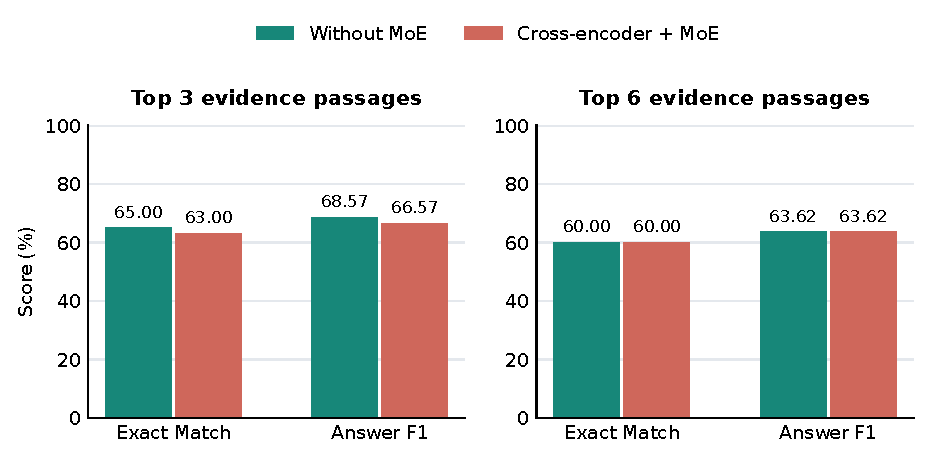
\includegraphics[width=0.94\linewidth]{01_answer_quality.pdf}
\caption{Answer EM and token F1 on the same 100 text questions. Both cutoffs use the same saved-candidate protocol. Axes start at zero; the top-3 reduction is two percentage points. Equal top-6 aggregate metrics do not imply identical per-question answers.}
\label{fig:mainresults}
\end{figure}

\begin{table}[htbp]
\centering
\small
\caption{Main factual QA results on 100 questions. Hit, EM, and F1 are percentages; MRR and nDCG use the 0--1 scale.}
\label{tab:results}
\begin{tabular}{@{}clrrrrr@{}}
\toprule
$K$ & Condition & Hit (\%) & MRR & nDCG & EM (\%) & F1 (\%)\\
\midrule
3 & Without MoE & 95.00 & 0.9267 & 0.9326 & 65.00 & 68.57\\
3 & Cross-encoder + MoE & 95.00 & 0.9200 & 0.9276 & 63.00 & 66.57\\
\midrule
6 & Without MoE & 98.00 & 0.9323 & 0.9439 & 60.00 & 63.62\\
6 & Cross-encoder + MoE & 98.00 & 0.9262 & 0.9394 & 60.00 & 63.62\\
\bottomrule
\end{tabular}
\end{table}

At top 3, MoE reduces EM by two percentage points and F1 by two points while leaving Hit unchanged. At top 6, both conditions have the same EM and F1, although MRR and nDCG are slightly lower with MoE. The full candidate order changes for 99 of 100 questions. At top 3, 54 rankings and 39 evidence sets change; eight answer strings change, with two previously exact answers becoming incorrect and none becoming exact.

\begin{figure}[htbp]
\centering
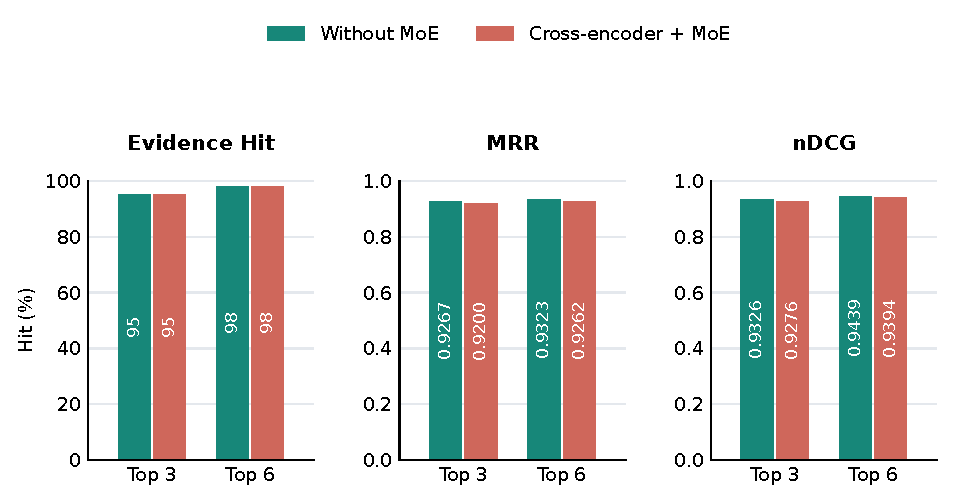
\includegraphics[width=0.94\linewidth]{02_evidence_ranking.pdf}
\caption{Evidence ranking at top 3 and top 6. MRR and nDCG use their full 0--1 scale, with numerical annotations to show the small differences. Equal aggregate Hit does not imply identical retrieved evidence.}
\label{fig:rankingresults}
\end{figure}

\subsection{Subgroup results}
\begin{table}[htbp]
\centering
\small
\caption{Top-3 answer F1 by target source and modality.}
\label{tab:subgroups}
\begin{tabular}{@{}lrrr@{}}
\toprule
\textbf{Stratum} & \textbf{Baseline} & \textbf{Cross-encoder + MoE} & \textbf{Difference}\\
\midrule
DOSA ($n=20$) & 71.43 & 71.43 & 0.00\\
SCALE ($n=20$) & 47.26 & 42.26 & $-5.00$\\
DRISHTIKON ($n=20$) & 85.00 & 85.00 & 0.00\\
DIWALI ($n=20$) & 77.50 & 72.50 & $-5.00$\\
Indian Cultural Dataset ($n=20$) & 61.67 & 61.67 & 0.00\\
\midrule
Text-only targets ($n=80$) & 64.46 & 61.96 & $-2.50$\\
Image-associated targets ($n=20$) & 85.00 & 85.00 & 0.00\\
\bottomrule
\end{tabular}
\end{table}

The largest subgroup reductions occur in SCALE and DIWALI. Equal scores on image-associated questions do not prove that image features improve ranking; this is a source-modality breakdown, not a controlled image-masking experiment. The paired source-group bootstrap interval for the top-3 F1 difference (MoE minus baseline) is approximately $[-5.10,0.00]$ percentage points, which does not support a clear advantage.

\begin{figure}[htbp]
\centering
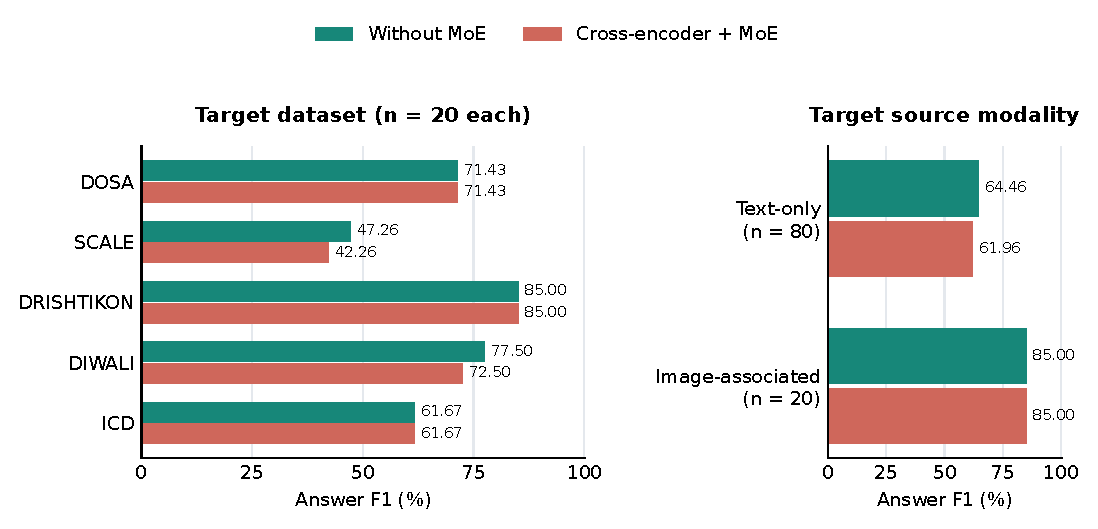
\includegraphics[width=0.94\linewidth]{03_subgroup_quality.pdf}
\caption{Top-3 answer F1 by target dataset (20 questions each) and target-source modality (80 text-only and 20 image-associated questions). ICD denotes the Indian Cultural Dataset. These strata are not a controlled image-masking experiment.}
\label{fig:subgroupresults}
\end{figure}

\subsection{Shared Image Retrieval and Processing Cost}
The shared CLIP image retrieval path achieved Hit of 85\% at top 3 and 95\% at top 6 over 20 image queries. No improvement from MoE is claimed for this image-retrieval path. In the main replay, frozen fusion-feature extraction averaged 0.971 seconds per text query and learned reranking 0.009 seconds. This approximately 0.98-second fusion component is not a fresh end-to-end latency measurement.

\section{Discussion}
The current MoE design does not improve the measured answer metrics over the cross-encoder baseline. A plausible explanation is that hybrid retrieval and the pretrained cross-encoder already provide a strong relevance signal; at top 6, the candidate set contains labelled evidence for 98\% of questions, leaving limited headroom. The MoE was trained on 300 weakly supervised anchors and one seed. Further, four of the five sources contain only text; on candidates without an image, the model combines text transformations with a learned constant image projection. This source breakdown does not establish the image availability of every retrieved candidate pool.

The result does not show that MoE is inherently unsuitable for cultural retrieval. It shows that this specific model, supervision, and ranking combination did not improve the measured benchmark. The practical choice for this version is to retain cross-encoder ranking, improve long-record indexing and labels, and evaluate future fusion models on a new independently reviewed benchmark. The decrease in EM when increasing $K$ from 3 to 6, despite higher evidence Hit, also suggests that reader selection and context quantity deserve attention.

\section{Limitations}
The benchmark contains only 100 factual questions and 20 image queries and had been inspected previously. Training labels are weak, only one training seed was used, and relevance judgements are incomplete. The saved replay is not a fresh end-to-end blind evaluation, and the bootstrap interval does not capture annotation error or seed variance. The experiment does not isolate expert mixing from extra parameters, training, and image access. The Indian Cultural Dataset is incompletely indexed, and image-associated records occur only in DRISHTIKON. Exact Match and token F1 do not fully measure cultural validity or semantic equivalence. A new independently reviewed evaluation set, multiple seeds, controlled image-masking, and parameter-matched fusion baselines are needed before broader conclusions can be drawn.

\section*{Ethics and Responsible Use}
Cultural sources can reflect the perspectives and omissions of their creators. Retrieved evidence should be treated as support to inspect, not proof of correctness. Coverage varies across sources, particularly because only 4.24\% of the Indian Cultural Dataset's characters are indexed. Dataset and model licences remain with their providers. Query expansion sends user questions to a third-party API, which should be considered when handling sensitive queries.

\section{Conclusion}
CulturalQA combines hybrid retrieval, cross-encoder reranking, and extractive reading over five cultural resources, with a separate CLIP image-retrieval path. In a matched saved-candidate replay, adding the MoE fusion score did not improve answer quality: top-3 EM and F1 fell from 65\% and 68.57\% to 63\% and 66.57\%, while top-6 EM remained 60\%. We therefore retain the cross-encoder as the strongest measured configuration for this benchmark. The results are preliminary and motivate improved indexing, stronger supervision, controlled ablations, and independent evaluation.

%*\section*{Acknowledgments}
%The authors should add any funding, compute-resource, and other acknowledgments before submission.
%\section*{Author Contributions}
%Add a brief contribution statement assigning conceptualization, implementation, experiments, analysis, and writing roles accurately before submission.%

\begingroup
\small
\begin{thebibliography}{30}
\bibitem{rag} P. Lewis et al. ``Retrieval-Augmented Generation for Knowledge-Intensive NLP Tasks.'' NeurIPS, 2020. \url{https://arxiv.org/abs/2005.11401}
\bibitem{sbert} N. Reimers and I. Gurevych. ``Sentence-BERT: Sentence Embeddings using Siamese BERT-Networks.'' EMNLP-IJCNLP, 2019. \url{https://aclanthology.org/D19-1410/}
\bibitem{bm25} S. Robertson and H. Zaragoza. ``The Probabilistic Relevance Framework: BM25 and Beyond.'' \emph{Foundations and Trends in Information Retrieval}, 3(4):333--389, 2009.
\bibitem{rrf} G. V. Cormack, C. L. A. Clarke, and B. Buettcher. ``Reciprocal Rank Fusion Outperforms Condorcet and Individual Rank Learning Methods.'' SIGIR, 2009.
\bibitem{faiss} J. Johnson, M. Douze, and H. J\'egou. ``Billion-scale Similarity Search with GPUs.'' arXiv:1702.08734, 2017. \url{https://arxiv.org/abs/1702.08734}
\bibitem{monobert} R. Nogueira and K. Cho. ``Passage Re-ranking with BERT.'' arXiv:1901.04085, 2019. \url{https://arxiv.org/abs/1901.04085}
\bibitem{msmarco} P. Bajaj et al. ``MS MARCO: A Human Generated MAchine Reading COmprehension Dataset.'' arXiv:1611.09268, 2016. \url{https://arxiv.org/abs/1611.09268}
\bibitem{roberta} Y. Liu et al. ``RoBERTa: A Robustly Optimized BERT Pretraining Approach.'' arXiv:1907.11692, 2019. \url{https://arxiv.org/abs/1907.11692}
\bibitem{squad1} P. Rajpurkar et al. ``SQuAD: 100,000+ Questions for Machine Comprehension of Text.'' EMNLP, 2016. \url{https://aclanthology.org/D16-1264/}
\bibitem{squad2} P. Rajpurkar, R. Jia, and P. Liang. ``Know What You Don't Know: Unanswerable Questions for SQuAD.'' ACL, 2018. \url{https://aclanthology.org/P18-2124/}
\bibitem{shazeer} N. Shazeer et al. ``Outrageously Large Neural Networks: The Sparsely-Gated Mixture-of-Experts Layer.'' ICLR, 2017. \url{https://arxiv.org/abs/1701.06538}
\bibitem{switch} W. Fedus, B. Zoph, and N. Shazeer. ``Switch Transformers: Scaling to Trillion Parameter Models with Simple and Efficient Sparsity.'' JMLR, 2022. \url{https://arxiv.org/abs/2101.03961}
\bibitem{tfn} A. Zadeh et al. ``Tensor Fusion Network for Multimodal Sentiment Analysis.'' EMNLP, 2017. \url{https://aclanthology.org/D17-1115/}
\bibitem{lmf} Z. Liu et al. ``Efficient Low-rank Multimodal Fusion with Modality-Specific Factors.'' ACL, 2018. \url{https://aclanthology.org/P18-1209/}
\bibitem{retvqa} A. S. Penamakuri, M. Gupta, M. Das Gupta, and A. Mishra. ``Answer Mining from a Pool of Images: Towards Retrieval-Based Visual Question Answering.'' IJCAI, 2023. \url{https://arxiv.org/abs/2306.16713}
\bibitem{bert} J. Devlin et al. ``BERT: Pre-training of Deep Bidirectional Transformers for Language Understanding.'' NAACL, 2019. \url{https://aclanthology.org/N19-1423/}
\bibitem{clip} A. Radford et al. ``Learning Transferable Visual Models From Natural Language Supervision.'' ICML, 2021. \url{https://proceedings.mlr.press/v139/radford21a.html}
\bibitem{dosa} Microsoft. ``DOSA dataset repository.'' \url{https://github.com/microsoft/DOSA}
\bibitem{scale} Google Research. ``SCALE Cultural Data.'' \url{https://github.com/google-research-datasets/SCALE-Cultural-Data}
\bibitem{diwali} NLIP. ``DIWALI dataset.'' \url{https://huggingface.co/datasets/nlip/DIWALI}
\bibitem{drishtikon} ``DRISHTIKON dataset.'' \url{https://huggingface.co/datasets/13ari/DRISHTIKON}
\bibitem{icd} ``Indian Cultural Dataset.'' \url{https://huggingface.co/datasets/ombhojane/indian-cultural-dataset}
\end{thebibliography}
\endgroup

\end{document}
